\documentclass{article}
\usepackage{tikz}

\newcommand{\nl}{\\[6pt]}

\begin{document}
\title{Abstract argumentation frameworks - overview and illustration}
\author{Patrick Bellositz}
\date{}
\maketitle

\section{Introduction}

\section{Definitions}
\textbf{Definition 1} An \emph{argumentation framework} $F$ is a pair $(A,R)$, where $A$ is a set of arguments and $R$ is a set of attack relations.\nl
\textbf{Definition 2} \emph{Attack relations} $R\subseteq A\times A$ represent attacks. The pair $(a,b)$, where $a,b\in A$ means $a$ \emph{attacks} $b$.\nl
\textbf{Remark 1} Let $S$ be a set of arguments. If $a\in S$ and there is an attack $(a,b)\in R$ we say $S$ \emph{attacks} $b$.\nl
\textbf{Definition 3} Let $S$ be a set of arguments. It is \emph{conflict-free}, if $\forall a \forall b\ a,b\in S, (a,b)\notin R$.\nl
\textbf{Definition 4} An argument $a$ is \emph{defended} by a set $S$, if for every attack $(b,a)\in R$ there is an attack $(c,b)$, where $c\in S$. If this is the case $S$ \emph{defends} $a$.\nl
\textbf{Definition 5} Let $S$ be a conflict-free set. It is called an \emph{admissible extension} if it defends each $a\in S$.\nl
\textbf{Definition 6} Let $S$ be an admissible extension. It is called a \emph{preferred extension} if for each $S'\subseteq A$, that is an admissible extension, $S\not\subset S'$.\nl
\textbf{Definition 7} Let $S$ be a conflict-free set. It is called a \emph{stable extension} if for each $a\not\in S$ there is exists an attack $(b,a)\in R$ where $b\in S$.\nl
\textbf{Definition 8} Let $S$ be an admissible extension. It is called a \emph{complete extension} if for each $a\not\in S$, $S\cup \{a\}$ is not an admissible extension.\nl
\textbf{Definition 9} The (unique) \emph{grounded extension} is defined by $\bigcap\limits_{i=1}^n{S_i}$, where $\{S_1,...,S_n\}$ is the set of all complete extensions.\nl

\section{Observations}
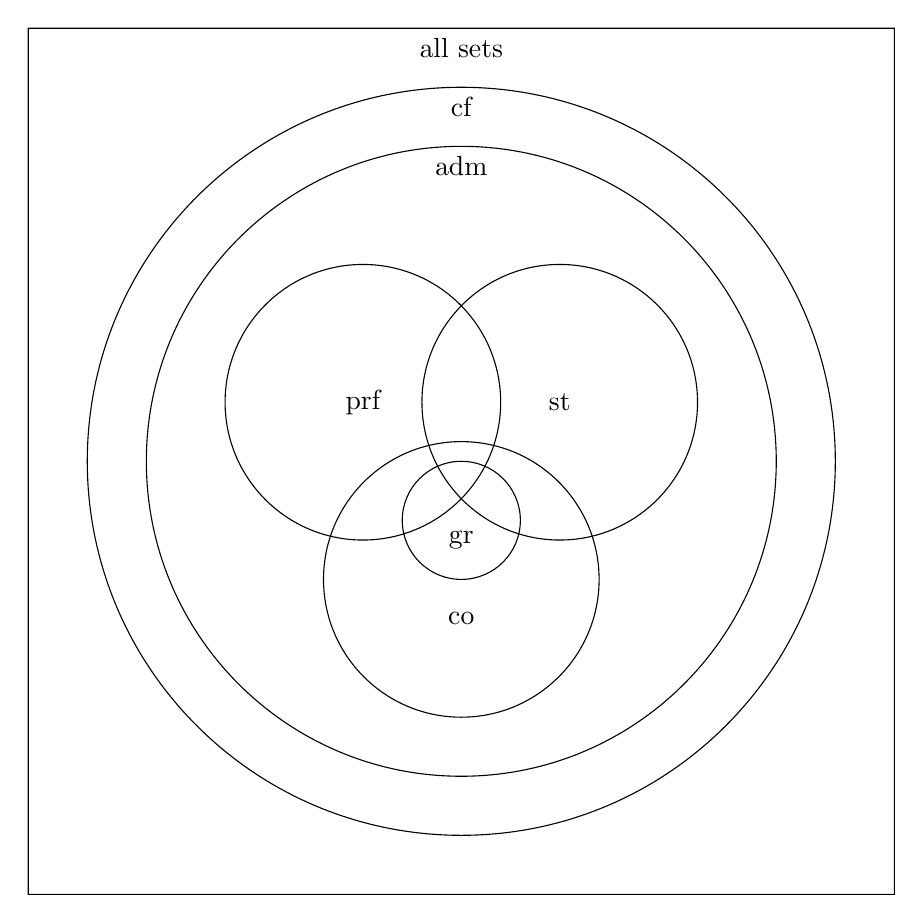
\begin{tikzpicture}[fill=white]
% left hand
\scope
\clip (-2,-2) rectangle (2,2)
      (1,0) circle (1);
\fill (0,0) circle (1);
\endscope
% right hand
\scope
\clip (-2,-2) rectangle (2,2)
      (0,0) circle (1);
\fill (1,0) circle (1);
\endscope
% (xpos,ypos) circle (radius) (textx,texty) [modifiers] {text}
\draw (3.5,3.5) circle (4.75) (3.5,7.75) node [text=black,above] {cf}
	 (3.5,3.5) circle (4) (3.5,7) node [text=black,above] {adm}
	 (2.25,4.25) circle (1.75) node [text=black] {prf}
	 (4.75,4.25) circle (1.75) node [text=black] {st}
	 (3.5,2) circle (1.75) (3.5, 1.5) node [text=black] {co}
	 (3.5,2.75) circle (.75) (3.5, 2.5) node [text=black] {gr}
     	 (-2,-2) rectangle (9,9) (3.5,8.75) node [text=black]{all sets};
\end{tikzpicture}

\section{Application}
\subsection{Introduction}
In this section the usage and implementation details of the aforementioned program illustrating the computation of the different extension types is provided.

\subsection{Creation of a framework}

\subsection{Argumentation graph}

\subsection{stuff comes here}

\end{document}
